%!TEX root = main.tex

\section{Understanding Voice Recognition Performance}
\label{sec:voice}

\begin{table*}[t]
\caption{High-level statistics of voice recognition flows.}
\label{tab:voice_stats}
\centering
\renewcommand{\arraystretch}{1.0}
\begin{tabular}{c|C{2.6cm}|c|c|C{2.1cm}|C{2.1cm}}
	\hline
	& Flow completion time (ms) & Flow size (\#pkts) & RTT (ms) & \% of flows w/ reord. pkts & \% of flows w/ timeout retx \\
	\hline
	WiFi & 69 (15, 1,052) & 3.0 (2.0, 4.0) & 45 (12, 399) & 3.3\% & 9.5\% \\
	%\hline
	3G & 55 (6, 316) & 3.0 (2.0, 4.0) & 35 (5, 99) & 6.6\% & 7.3\% \\
	\hline
\end{tabular}
\minsqueeze
\end{table*}

%\begin{figure}[th]
%	\centering
%	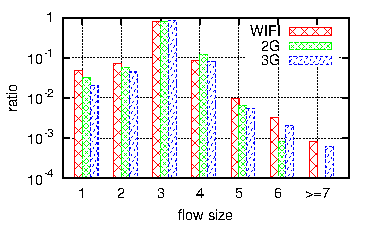
\includegraphics[width=0.8\linewidth]{voice_flow_size}
%	\caption{The number of voice data packets in voice recognition flows.}
%	\label{fig:voice_flow_size}
%\end{figure}

In this section, we look at TCP performance of voice recognition flows. We first provide high-level statistics on key performance indicators for 3G and WiFi flows in Table~\ref{tab:voice_stats}. For flow completion time, flow size and RTT, we report the median along with the $5th$ and $95th$ percentiles in parenthesis. The flow size is measured in number of data packets. Independent of the access technology, nearly all voice recognition flows contains no more 4 data packets. Given that the initial congestion window in the current Android TCP/IP stack is set to 10 segments~\cite{dukkipati2010argument}, the data can be transmitted in the initial congestion window. Another interesting observation from Table~\ref{tab:voice_stats} is that 3G flows tend to have smaller RTTs but a higher probability of suffering from packet reordering. In what follows, we examine each TCP performance factor and its impact on the flow completion time.

\subsection{RTT}

As illustrated in Figure~\ref{fig:voice_estimate_rtt}, we can measure at most 3 RTTs at the server-side in a voice recognition flow. However, the RTT is ambiguous when segments are retransmitted. To address this, we use the following methodology to determine the \emph{minimal RTT}. If no retransmission happens for SYN packets, $t^s_a - t^s_s$ is used as the RTT of the flow, \ie the RTT is measured during the 3WHS (3-way handshake). Otherwise, the RTT measured during connection termination is preferred if the FIN packet is not retransmitted. In the case that both of the above RTTs are ambiguous, $t^s_t - t^s_r$ is used as the measured RTT. We have verified using our datasets that the RTT measured during 3WHS is the minimal RTT in more than 60\% of flows, and is less than 2 times of the minimal RTT in 95\% of flows. We believe that it is reasonable to assume that the RTT measured using the above methodology is close to the minimal RTT of the flow, and the most representative of the network latency.

Figure~\ref{fig:voice_rtt} plots the distribution of RTTs measured in individual voice recognition flows. The median RTT of 3G flows is around 35 ms. WiFi flows on the other hand exhibit a larger RTT with a median around 45 ms. In particular, while 95\% of 3G flows have a RTT less than 100 ms, about 20\% of WiFi flows have a RTT larger than this value.

\begin{figure}[t]
\centering
	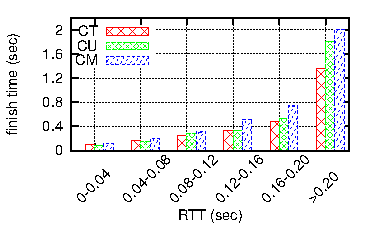
\includegraphics[width=0.8\linewidth]{voice_rtt}
\caption{RTTs in voice recognition flows.}
\label{fig:voice_rtt}
\minsqueeze
\end{figure}

\begin{figure}[th]
\centering
	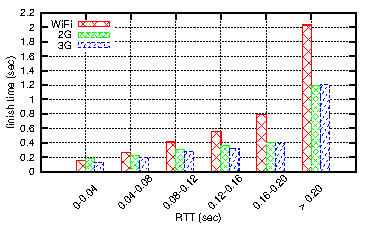
\includegraphics[width=0.8\linewidth]{voice_rtt_finish_time}
\caption{Impact of RTT on flow completion time for voice recognition flows.}
\label{fig:v_rtt_time}
\minsqueeze
\end{figure}

We further examine the impact of RTT on flow completion time in Figure~\ref{fig:v_rtt_time}. We observe that for flows having a RTT no larger than 200 ms, the flow completion time increases with the RTT: the ratio of flow completion time to RTT is about 2.5 for 3G flows and about 4 for WiFi flows. Since the completion time of a voice recognition flow is approximately 2 RTTs (in which 1 RTT for building connection, and 1 RTT for uploading data), the difference of the ratio between cellular network and WiFi network should come from the data uploading time. One possibility is that the RTT during data transfer in WiFi is significantly higher than the RTT measured during connection establishment (\ie 3WHS) \cite{UM-CS-2012-022}, where we obtained most of the RTTs. It seems that 3G networks provide consistent RTTs during the flow lifetime.

The flow completion time becomes extremely large when the RTT is larger than 200ms. Such an RTT could be an indication of network congestion, as the servers are likely to be geographically close to the clients. In other words, it is likely that the flow is traversing a congested network and may encounter packet loss, which may take a relatively long time for recovery.

\subsection{Packet Reordering}
\label{sec:v_pd}

\begin{figure*}[th]
\centering
	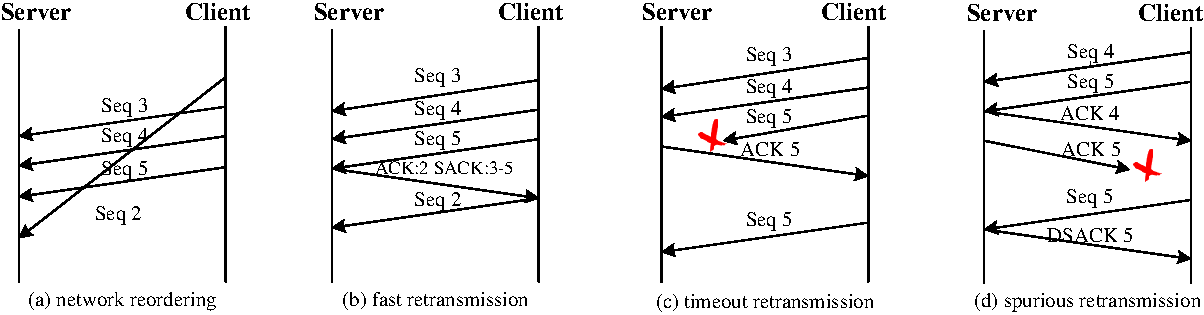
\includegraphics[scale=0.7]{voice_flow_estimate_retrans}
\caption{Server could not distinguish packet reordering events, which are (a) packet reordering, (b) fast retransmit, and (c) timeout retransmission. Server may identify some timeout retransmissions as long packet delay (d).}
\label{fig:voice_flow_estimate_retrans}
\minsqueeze
\end{figure*}

Another factor that can heavily impact the flow completion time are network congestion events, which can be observed by servers as packet loss, packet delay and packet reordering. However, as a TCP receiver, the server might not be able to infer the type of network congestion event. For example, the server observes the same packet sequences for Figure~\ref{fig:voice_flow_estimate_retrans}(a), \ref{fig:voice_flow_estimate_retrans}(b) and \ref{fig:voice_flow_estimate_retrans}(c), despite that they depict 3 types of congestion: packet reordering in Figure~\ref{fig:voice_flow_estimate_retrans}(a), fast retransmit for packet loss recovery in Figure~\ref{fig:voice_flow_estimate_retrans}(b) and timeout retransmission for packet loss recovery in Figure~\ref{fig:voice_flow_estimate_retrans}(c). These observations illustrate the challenge in TCP analysis from the server-side.

We use the number of reordered packets, a metric that the server can compute, to capture the network congestion characteristics. In the examples shown in the first 3 subfigures in Figure~\ref{fig:voice_flow_estimate_retrans}, the number of reordered packets is 1. %As we have shown in Figure~\ref{fig:voice_flow_estimate_retrans}, a reordered packet seen by the serve could be caused by either packet reordering, fast retransmit or timeout retransmission for packet loss recovery (i.e. Figure~\ref{fig:voice_flow_estimate_retrans}(a-c)). 
We report the percentage of flows with packet reordering in Table~\ref{tab:voice_reorder}.

\begin{table}[th]
\caption{Percentage of flows with packet reordering.}
\label{tab:voice_reorder}
\centering
\renewcommand{\arraystretch}{1.0}
\begin{tabular}{c|c|c|c}
	\hline
	\# reord. pkts & 0 & 1 & $\ge$2 \\
	\hline
	WiFi & 96.7\% & 3.03\% & 0.2\% \\
	\hline
	3G & 93.3\% & 6.6\% & - \\
	\hline
\end{tabular}
\minsqueeze
\end{table}

As expected, the majority of flows experience no packet reordering. However, we observe that 6.6\% of 3G flows and 3\% of WiFi flows have one reordered packet. The fraction of flows having more than 2 reordered packets is negligible. Given that in most cases, the voice data only consists of 3 packets, just a single reordered packet can severely impair flow performance as shown in Figure~\ref{fig:voice_reorder}.

\begin{figure}[th]
\centering
	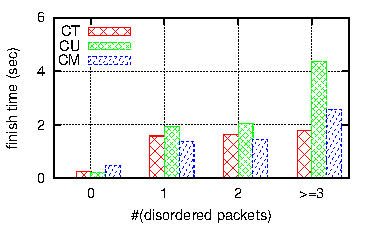
\includegraphics[width=0.8\linewidth]{voice_reorder}
\caption{Impact of packet reordering on flow completion time.}
\label{fig:voice_reorder}
\minsqueeze
\end{figure}

We can see from Figure~\ref{fig:voice_reorder} that one reordered packet in 3G uploading flows can increase the median flow completion time from 10 ms to 60 ms. For WiFi flows, we observe as many as 20\% of the flows suffering from packet reordering cannot finish the upload within 1 second. When receiving a reordered packet, the server feeds back to the client with a SACK (as shown in Figure~\ref{fig:voice_flow_estimate_retrans}). The client will retransmit the packet in the hole (\ie the reordered packet) after collecting 3 SACKs. In the case that too few SACKs can be collected, the client has to rely on the expensive timeout retransmission mechanism for recovery. %That said, the increased flow completion time might be caused by either packet delay, fast retransmit or timeout retransmission. Unfortunately, we cannot identify how much each of these congestion events contributes using the datasets collected from server side.

The significance of the impact of packet reordering on flow completion time is also dependent on RTT, as both the waiting time for fast retransmit and timeout retransmission timer (\ie RTO) depend on the RTT. To further assess the impact of packet reordering by excluding the possible effect of other covariates (\eg RTT), we rely on non-parametric factorial analysis using a Quasi Experimental Design (QED) \cite{krishnan2013video}. In QED, each uniformly sampled individual $u$ is compared with an individual $v$ randomly selected from those that have identical covariates with $u$ except the cause variable (packet reordering in our context). Any difference in outcome between these two individuals can be attributed to the cause variable we are tracking.

We bin for each access technology the voice recognition flows into two groups: those with no reordered packet ($G_1$) and those with 1 reordered packet ($G_2$). For each flow $u \in G_1$, we randomly choose a flow $v$ from $G_2$ that has similar RTT (\ie the difference is less than 40 ms) and the same condition in terms of timeout retransmission as identified by the methodology from Section~\ref{sec:v_rto}. We record the outcome difference as $o_{u,v} = \frac{ftime_{v} - ftime_{u}}{ftime_{u}}$, where $ftime_v$ is the completion time of the flow $v$. Finally, we average all outcome differences over the matched pairs and use this average difference to gauge the impact of packet reordering.

\begin{table}[th]
\caption{QED results for the impact of packet reordering.}
\label{tab:voice_qed_reorder}
\centering
\renewcommand{\arraystretch}{1}
\begin{tabular}{C{1cm}|C{1.5cm}|C{1.5cm}}
	\hline
	 & WiFi & 3G \\
	\hline
	QED & 6.42 & 4.45 \\
	\hline
\end{tabular}
\minsqueeze
\end{table}

Table~\ref{tab:voice_qed_reorder} presents the QED results, which show that one reordered packet can lead to an increase of flow completion time by a factor as large as $4-6$. The larger flow completion time increase of WiFi compared to 3G flows is due to the packet reordering events in WiFi flows that are more likely to originate in packet losses (\ie Figure \ref{fig:voice_flow_estimate_retrans}(b) and \ref{fig:voice_flow_estimate_retrans}(c)), which require more time to recover. Indeed, we find using the web search dataset that the packet loss rate in WiFi is 3.9\% compared to 0.9\% in 3G\footnote{We cannot obtain the packet loss rate of voice recognition flows as the server where we collected our dataset is a TCP receiver}. 

\subsection{Timeout Retransmissions}\label{sec:v_rto}

\begin{figure}[th]
\centering
	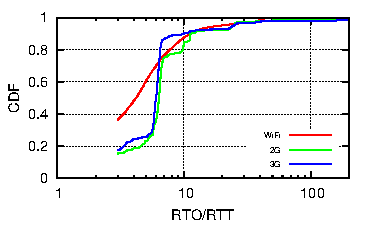
\includegraphics[width=0.8\linewidth]{voice_rtt_rto_ratio}
\caption{Distribution of RTO/RTT.}
\label{fig:rto_rtt}
\minsqueeze
\end{figure}

We rely on the time gap between actual arrival time and the estimated arrival time of individual packets to infer timeout retransmissions in voice recognition flows. We observe a behavior similar to Figure~\ref{fig:voice_flow_estimate_retrans}(d). The estimated arrival time of a packet is the mean value of the arrival time of the previous packet and subsequent packets. If this gap is larger than a RTO, the transmission of the packet is identified as a timeout retransmission. However, the server does not know the client-side RTO, which has to be estimated. The RTO in the TCP implementation is set to $\text{SRTT} + max(200ms, 4 \text{ RTTVAR})$\cite{rfc62982011computing}, where SRTT is close to RTT, and RTTVAR is approximately $RTT/2$, \ie $$\widehat{RTO} \approx RTT + max(200ms, 2 RTT) \enspace .$$ Note that the timeout retransmissions identified using the above methodology do not overlap with those shown in Figure~\ref{fig:voice_flow_estimate_retrans}(c).

We first examine how large RTOs can be in Figure~\ref{fig:rto_rtt}, where we plot the distribution of RTO/RTT. We can observe the median RTO is around 4-6 times the RTT, but can be as large as tens of or even hundreds of RTTs. Given that a time retransmission takes a RTO for recovery, the impact of timeout retransmission on flow completion time can be significant.

\begin{table}[th]
\centering
\renewcommand{\arraystretch}{1.1}
\caption{Flows with timeout retransmission.}
\label{tab:voice_timeout_stats}
\begin{tabular}{c | C{2cm} | C{2cm}}
	\hline
	 & WiFi & 3G \\
	\hline
	% packet reordering & 3.2\% & 5.6\% & 6.2\% \\
	% \hline
	3WHS retx & 2.6\% & 0.8\% \\
	%\hline
	data retx & 9.5\%  & 7.3\% \\
	% \hline
	% incomplete transmission & 0.2\% & 0.3\% & 2.4\% \\
	\hline
\end{tabular}
\minsqueeze
\end{table}

Table~\ref{tab:voice_timeout_stats} lists the percentage of flows that suffer from at least one timeout retransmission in our dataset. The timeout retransmission could happen either during the 3WHS or data transmission. While the timeout retransmission during 3WHS is less likely to happen compared to timeout retransmission during data upload, its impact might be even larger. This is because the initial RTO is set to 1 second~\cite{rfc62982011computing} as there is no RTT available at that time. This RTO value is often much larger than the one computed during data upload. Users might quit the app during this the period taken for recovery. In addition, a timeout retransmission during the 3WHS results in the congestion window size going to 1, which further impairs the performance for data transmission.

Regardless of the access technology, we observe as many as over 7\% of the voice data upload flows suffering from at least one timeout retransmission. Such a large fraction of timeout retransmission flows can be explained by the fact that almost all the voice recognition flows contain no more than 4 voice data packets. When one of the last three packets is dropped, the sender (\ie client) has to rely on RTO for retransmission. This behavior is similar to the tail loss identified in~\cite{flach2013reducing}. In the voice data upload context, the server is no longer a sender and thus unable to eliminate such kind of RTO retransmissions by gently sending redundant packets as proposed in~\cite{flach2013reducing}. Our results highlight the need for TCP optimizations at the server-side. 

\begin{figure}[th]
\centering
	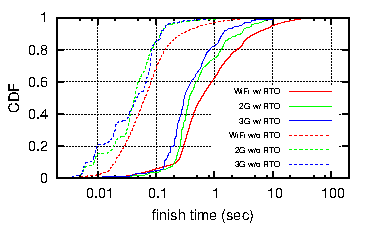
\includegraphics[width=0.8\linewidth]{voice_timeout}
\caption{CDF of flow completion time with and without timeout retransmission.}
\label{fig:voice_rto}
\minsqueeze
\end{figure}

\begin{table*}[t]
\caption{High-level statistics of web search flows.}
\label{tab:web_stats}
\centering
\renewcommand{\arraystretch}{1.0}
\begin{tabular}{c|C{2.6cm}|c|c|C{1.2cm}|C{1.85cm}|C{2.1cm}}
	\hline
	& {Flow completion time (ms)} & {flow size (\#pkts)} & {RTT (ms)} & pkt loss rate & \% of flows w/ lost pkts & \% of flows w/ timeout retx \\
	\hline
	WiFi & 197 (30, 4,608) & 9.0 (1.0, 33.0) & 39 (10, 372) & 3.0\% & 9.76\% & 4.1\% \\
	\hline
	3G & 124 (15, 440) & 19.0 (1.0, 82.0) & 38 (4, 68) & 0.9\% & 8.7\% & 0.1\% \\
	\hline
\end{tabular}
\minsqueeze
\end{table*}

We finally compare the completion time between flows with and without timeout retransmission in Figure~\ref{fig:voice_rto} (note the log scale $x$-axis). The timeout retransmission increases the median flow completion time from 64ms to 595ms, \ie one order of magnitude larger. This is not surprising given that RTO is several times larger than the RTT. Perhaps more importantly, we observe that 10\% of WiFi flows with timeout retransmissions require as much as 5 seconds to upload the voice data. The voice search sessions that correspond to these flows are indeed likely to be terminated by the user. In fact, since the number of voice data packets is relatively small ($\le 4$), which can be uploaded within 2 RTTs, the retransmission time (\ie RTO) will dominate the flow completion time of the flows experiencing timeout retransmissions.  Overall, a larger fraction of WiFi flows suffer from timeout retransmission compared to 3G flows, which partially explains their larger flow completion time observed in Figure~\ref{fig:voice_finish_time}.

\subsection{Summary of Voice Recognition Analysis}

The key observations on voice recognition flows are summarized as follows:
\begin{itemize}
\item Most of voice recognition flows contain no more than 4 data packets, which fit into the initial congestion window of the client. Ideally, the voice data can be transmitted in 1 RTT.
\item For flows with smaller RTT (say no more than 200 ms), the flow completion time is proportional to RTT. WiFi flows tend to have larger flow completion time compared to those in 3G, due to larger RTT. 	
\item Reordered packets, caused by either packet delay or packet loss, increasing the flow completion time by 4-6 times. Although WiFi flows are less likely to see reordered packets than 3G flows, they suffer more from packet reordering due to longer time for recovery.
\item Timeout retransmission, which can happen either during connection establishment or during data transfer, increases the flow completion time by as much as one order of magnitude. In addition, WiFi flows suffer more from timeout retransmissions than 3G flows.
\end{itemize}